\def\year{2015}
\documentclass[letterpaper]{article}
\usepackage{aaai}
\usepackage{times}
\usepackage{helvet}
\usepackage{courier}
\usepackage{graphicx}
\setlength\titlebox{3in}
\frenchspacing
\copyrighttext{Copyright 2015, California Institute of Technology}
\setlength{\pdfpagewidth}{8.5in}
\setlength{\pdfpageheight}{11in}
\pdfinfo{
/Title (Automatic Generation of a Mars Target Encyclopedia)
/Author (Kiri L. Wagstaff, Nina Lanza, Ellen Riloff, Chris Mattmann, Paul Ramirez)}
\setcounter{secnumdepth}{2}  
 \begin{document}
% The file aaai.sty is the style file for AAAI Press 
% proceedings, working notes, and technical reports.
%
\title{Automatic Generation of a Mars Target Encyclopedia}
\author{Kiri L. Wagstaff \\
Jet Propulsion Laboratory\\
California Institute of Technology\\
4800 Oak Grove Drive, Pasadena, CA 91109\\
{\tt kiri.l.wagstaff@jpl.nasa.gov}
\And
Nina L. Lanza\\
Los Alamos National Laboratory \\
Los Alamos, NM  87545\\
{\tt nlanza@lanl.gov}
\And
Ellen Riloff\\
School of Computing\\
University of Utah\\
Salt Lake City, UT 84112\\
{\tt riloff@cs.utah.edu}
\AND
Chris A. Mattmann\\ 
\normalsize Jet Propulsion Laboratory\\
\normalsize California Institute of Technology\\
\normalsize 4800 Oak Grove Drive, Pasadena, CA 91109\\
\normalsize {\tt chris.a.mattmann@jpl.nasa.gov}
\And
Paul M. Ramirez\\
\normalsize Jet Propulsion Laboratory\\
\normalsize California Institute of Technology\\
\normalsize 4800 Oak Grove Drive, Pasadena, CA 91109\\
\normalsize {\tt paul.m.ramirez@jpl.nasa.gov}
}
\maketitle
\begin{abstract}
\begin{quote}
TBD
\end{quote}
\end{abstract}

\section{Introduction and Motivation}

The surface exploration of Mars continues to generate new data and
discoveries for an increasingly large number of targets and locations.
Mission planners and planetary science researchers must be aware of an
ever-growing number of names, locations, and facts so that new
observations can be appropriately interpreted in the context of what
is already known.  For example, one might ask: Does the observation of
high manganese content at a particular location represent a
confirmation of an existing trend or an anomalous new discovery?

The rovers that have been sent to Mars have been extraordinarily
active and productive.  The Mars Science Laboratory rover has
generated $>3500$ targets in three years, and the Mars Exploration
rover has generated even more over its 11+-year mission.  There are
hundreds of associated scientific publications reporting new
discoveries.  The downside of this productivity is that as the number
of data and publications grow, it becomes progressively more difficult
for any single person to read, understand, organize, and recollect the
amount of information available.  All researchers face the challenge
of staying up to date on new methods and advances in their field, but
Mars surface studies are particularly challenging because rather than
learning about a handful of new methods every few months or so
(through a new journal issue or a conference proceedings), the list of
new targets and discoveries grows daily.

\begin{figure}
\centerline{\fbox{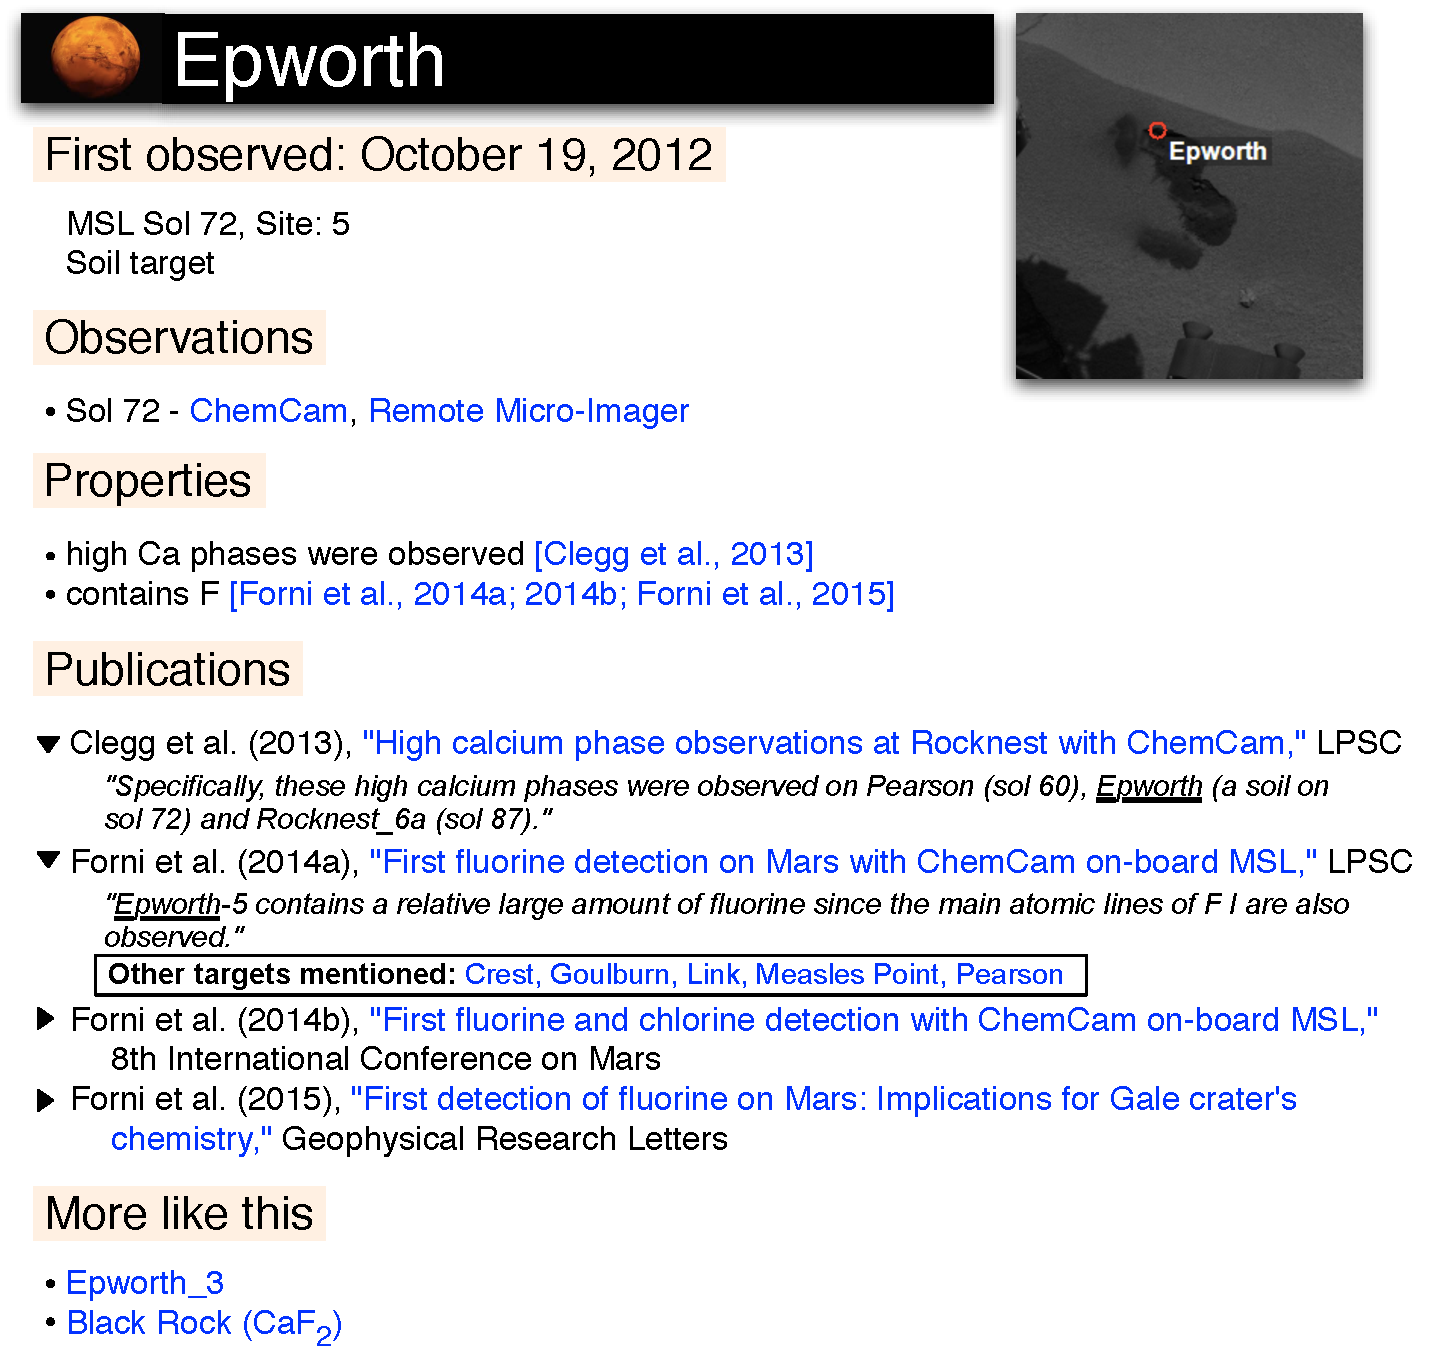
\includegraphics[width=3.25in]{fig/mte-epworth}}}
\caption{Example hand-constructed MTE entry for target
Epworth. Users can connect to the original observations, properties
that were extracted from scientific publications, and the publications
themselves.  Each publication provides excerpts with relevant context
and a list of other targets mentioned.}
\label{fig:epworth}
\end{figure}

There is a growing need for a comprehensive, up-to-date compilation of
Mars surface targets and what has been discovered about them.  The
number of targets, amount of data, and number of associated
publications are too large make this feasible as a manual task.
%
Current text search tools cannot meet the knowledge needs of planetary
scientists and mission planners.  Mars surface target names have no
naming convention, and names are often borrowed from Earth locations
(e.g.,~``Cumberland,'' ``Ithaca''), people (e.g., ``Jake'',
``Darwin''), or apparent whimsy (``Frood,'' ``Worldbeater'').  Using
Google or journal text search interfaces with these names yields many
irrelevant results.

%Volume of data: MSL - XXXX papers published in 3 years; YYYY targets
%observed by ChemCam

This situation presents an opportunity for NLP and information
extraction (IE) methods to make a major contribution that can help
advance the field of planetary science.  It also presents important
challenges that can motivate advances in IE that also benefit other
domains. 

We are working to construct a Mars Target Encyclopedia (MTE) that will
contain information about Mars surface targets.  The MTE will provide
access to the data and publications associated with each target (see
Figure~\ref{fig:epworth} for an example).  Each entry will also
include a list of properties that were automatically extracted from
the publications as a high-level summary of relevant knowledge.  The
associated excerpts will be highlighted for each publication, serving
to (1) provide support for each of the extracted properties and (2)
enable users to quickly determine which papers are of the most
interest.  Cross-document information extraction could also reveal new
connections or similarities between targets. {\bf [Cite Radev 00? Or
is this overkill?]}


\section{Constructing a Mars Target Encyclopedia}

\subsection{Corpus Description}

For our initial study, we constructed a corpus that consists of all
papers presented at the 2015 Lunar and Planetary Science Conference.
These papers consist of two-page extended abstracts that follow a
common structure: title, authors with affiliations, a two-column main
body that may contain figures and/or tables, and references.  The
language is academic and makes heavy use of complex noun phrases and
parenthentical expressions.  The passive voice is often used.
% Todo: include examples

% target list

\subsection{Approach}
- Sundance/Autoslog, Solr (?) database, JSON/webpage generation

- Use figure(s) from proposal to illustrate system operation

\begin{figure}
\centerline{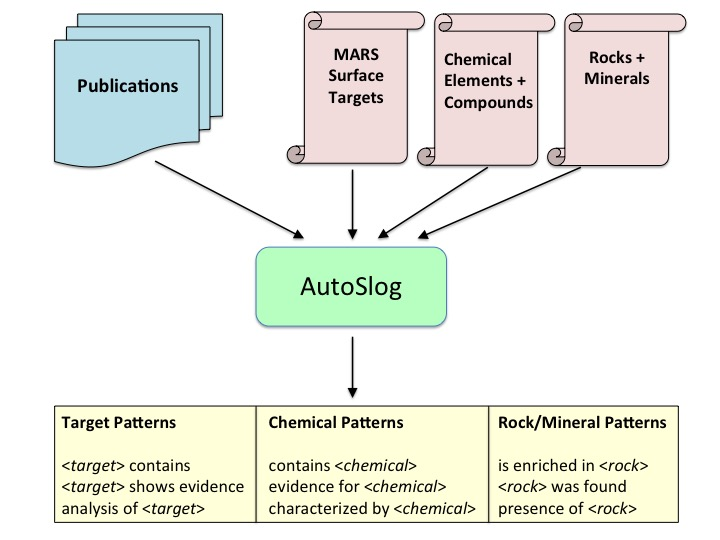
\includegraphics[width=3.5in]{fig/autoslog-process.jpg}}
\caption{The extraction pattern generation process. Autoslog learns
patterns from publications and lists of target names, chemical
elements and compounds, rocks, and minerals. {\bf [Ellen, this figure
looks a bit fuzzy - can we get a higher quality one, maybe PNG or PDF?]}}
\label{fig:ie}
\end{figure}

- domain-specific things we did

- lightly supervised? human review of extracted info - any annotations needed?

\subsection{Initial Results}

In this section, we report on initial results for extracting
information for a Mars surface target named Windjana.  Windjana is a
sandstone that was named after the Windjana Gorge in Western
Australia~\cite{}. 
% Cite paper 2417; this paper also has an nice image we could use

% todo: show parse output?
{\bf [Here we could show parse output and walk through one or more of
these examples.  Which one(s) should we use?]}

{\em ``Windjana is remarkable in containing an abundance of potassium
feldspar (and thus K in its bulk chemistry) combined with a low
abundance of plagioclase (and low Na/K in its chemistry).''}
% cite paper 2620
Autoslog extracts:
{\tt <subj>\_CONTAINING\_ABUNDANCE} 
(of potassium feldspar)

{\em ``As in other rock samples analyzed by CheMin, Windjana contains
significant proportions of phyllosilicates and amorphous material.''}
% cite paper 2620
Autoslog extracts:
{\tt <subj>\_CONTAINS\_PROPORTIONS}
(of phyllosilicates and amorphous material)

{\em ``The high abundances of K-feldspar and iron oxides in Windjana, also
reflected in the APXS chemical analysis as high K and Fe (Table 2)
[7], are unusual.''}
% cite paper 2620
Autoslog extracts:
(K-feldspar and iron) 
{\tt OXIDES\_IN\_<subj>}

{\em ``The Windjana sandstone contains high magnetite along with 2:1
phyllosilicates [9].''}
% cite paper 2971
Autoslog extracts:
{\tt <subj>\_CONTAINS\_MAGNETITE}
% need to know high/low!

\section{Challenges}

In addition to the typical challenges of conducting information
extraction in a new domain (e.g.,~domain-specific vocabulary), there
are several challenges of special interest involved in this project.

- need to combine case frames due to complex sentence structure

``strong enrichment in Zn on Windjana drill fines''



- New papers continually published; need automatic updating

- Reconcile potential conflicting information extracted from different
  authors and publications; knowledge evolves and some becomes
  outdated

- handle epistemic modifiers~\cite{sokolova:epistemic}. {\bf [Could
  also build on Ellen's previous work on subjective expressions?
  (EMNLP 2003)]} 

Examples:

``the Windjana drill tailings likely contain a spectrally opaque
material (e.g., magnetite, ilmenite)'' 

``the potential presence of illite in Windjana''

\section{Conclusions and Next Steps}

There is a need for an MTE

We can use IE tools, plus human review/vetting, to create a reliable
resource for planetary science 

  Benefits ongoing science
investigations and analysis of previously collected data within full
context.

We have not yet addressed the issue of coreference.

Expand to include more text sources and ultimately targets from other
instruments/missions 

\bibliography{mte}
\bibliographystyle{aaai}

\end{document}
